\subsection{Analog-to-Digital Converter} \label{sec:ADC_imp}
Mikrokontrolleren indeholder en SAR ADC, som gør det muligt at konvertere det analoge signal til et digitalt. Der ønskes en konfigurering af 3 analoge kanaler, herunder Y-aksen på begge accelerometre samt EMG-forstærkeren. Opsætningen af ADC'en på mikrokontrolleren fremgår af \autoref{fig:ADC_teori}. Det ønskes at kunne læse signalerne ved at måle single ended, hvorfor hvert input er tilkoblet $V_{ss}$, der fungerer som jord. Da der ligeledes ønskes at anvende en 12 bits-ADC på baggrund af kravet i \autoref{sec:ADC_teori}, indstilles denne til en opløsning på 12 bit. Da der anvendes en single ended konfiguration af kanalerne, svarer dette til, at ADC'en anvender 11 bit. ADC'en har et arbejdsområde fra $0-5~V$ \citep{ADC2014}. LSB'en for ADC'en kan beregnes ud fra \autoref{equ:LSB}, hvilket giver $2,44~mV$. Hvis der sker ændringer i signalet, der er mindre end LSB på $2,44~mV$, vil dette ikke komme til udtryk i det konverterede signal. 


\begin{figure}[H]
\centering
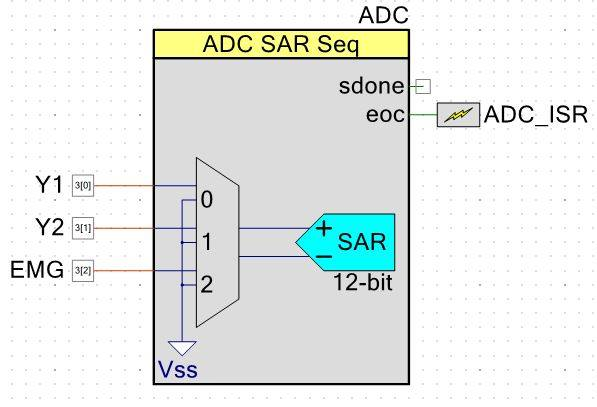
\includegraphics[width=0.5\textwidth]{figures/implementering/ADC_imp.jpg}
\caption{ADC'ens opsætning på PSoC. Sucessive Approximation Register (SAR) er typen af ADC. Kanalerne Y1, Y2 og EMG er de kanaler, der modtager signaler fra henholdsvis accelerometret, der er placeret på femur, accelerometret, der er placeret på tibia, og EMG-signal. sdone er en outputterminal, der signalerer, at ADC'en har samplet det aktuelle input. eoc signalerer, når en konversionscyklus er gennemført, dermed kan værdierne fra de samplede kanaler aflæses i samplingsregistret. Når eoc signalerer dette, laver ADC\_ISR et interrupt, der igangsætter endnu en læsning af kanalerne \citep{ADC2014}.}
\label{fig:ADC_teori}
\end{figure}

\noindent
I ADC'en er der indbygget en clock frekvens. Det er muligt at reducere konverteringstiden ved at øge ADC'ens clock frekvens, der kan indstilles mellem $1000~MHz$ og $9000~MHz$ \citep{ADC2014}. Clock cycles betegner tiden mellem to efterfølgende impulser fra en oscillator, og samplingtiden måles i clock cycles. Der er forskellige parametre, der kan indstilles i PSoC, herunder opløsning, samplingsrate og clock frekvens. Disse parametre bestemmer ADC'ens konverteringsrate. Konvertingstiden er den inverse af konverteringsraten. 

Da der ønskes at samples med 10 gange det opsamlede signals frekvensområde, hvilket i følge \autoref{sec:pilotforsoeg} er mellem 0,4 og $10~Hz$, vælges der at samples med $100~Hz$. Clockfrekvensen vælges til at have en hastighed på $1600~kHz$, hvilket svarer til en samplingsfrekvens på $100~Hz$ - \textbf{MADS - hvorfor var det nu???}. Som det fremgår af \autoref{fig:ADC_teori}, og figurteksten dertil, er outputtet fra ADC'en tilkoblet via eoc til ADC'ens Interrupt Service Routine (ISR). Hvis der er sker et interrupt vil dette resultere i, at de aktiverede kanaler er klar til at blive aflæst fra registrene, hvorved AD-konverteringen igangsættes \citep{ADC2014}.


